\section{需求分析与调研}

\subsection{需求分析}

根据题目描述,我们需要实现一个“更加智能的 Flash 文件系统”。

Flash介质因本身的擦除特性,给上层文件系统带来与普通磁盘、内存文件系统不同的数据管理模式。
同时,Flash的写入放大、寿命以及后期稳定性下降等问题也给文件系统的设计带来的一定的挑战。
传统的Flash文件系统并没有很好地解决这些稳定性相关问题。
这里希望寻找一种更智能、更合适的Flash文件系统设计,来更好地平衡Flash的性能与稳定性。
可以思考的方向包括但不限于:数据压缩算法(可以是自适应的压缩算法),检错、纠错、纠删码(可以是联合信源信道编码),数据块选择、擦除策略,Cache机制。

结合赛题内容,我们需要完成的文件系统需要具备以下特性:

\begin{itemize}
  \item {\bf{适合 Flash 介质}}:文件系统需要能够适应并缓解 Flash 的写入放大、寿命、后期稳定性等诸多 Flash 存储介质特有的问题
  \item {\bf{更智能}}:文件系统需要使用多种策略,在软件算法层面平衡性能与寿命
\end{itemize}

\subsubsection{往年实现分析}

本题在去年已经有队伍完成,他们的仓库在 \url{https://gitlab.eduxiji.net/why/project788067-124640}。
在选题之时,我们对其进行了调研。

他们队伍完成了一个基于 UBIFS 的适用于裸 Flash 设备的 YOUBIFS 文件系统,从以下几个方面对其进行了优化:

\begin{itemize}
  \item {\bf{数据压缩模块}}:使用了预压缩和自适应压缩结合的方法,均衡压缩比和写入速度
  \item {\bf{纠错编码模块}}:实现自适应生命周期、CRC+RAID5两种纠错方案
  \item {\bf{Cache 机制}}:添加读写缓冲
  \item {\bf{冷热数据识别}}:使用了冷热识别的纠错以提高 I/O 速度
\end{itemize}

\begin{figure}[htbp]
  \centering
  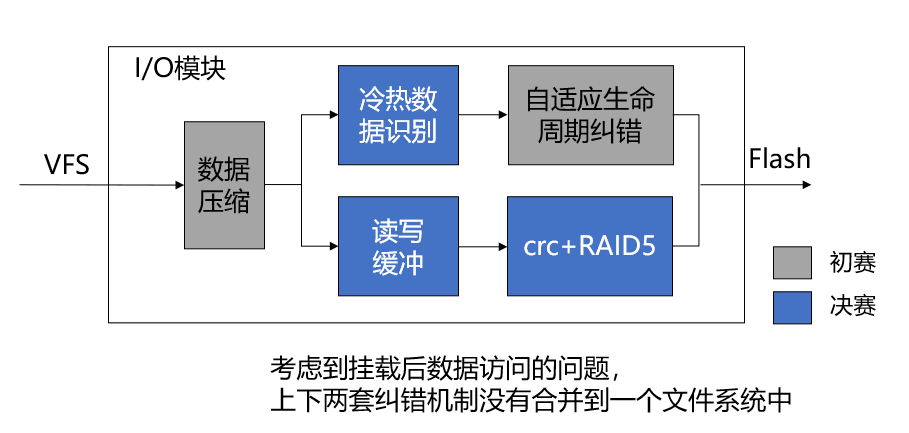
\includegraphics[width=0.7\textwidth]{fig/YOUBIFS项目框图}
  \caption{YOUBIFS 系统架构}
  \label{youbifs}
\end{figure}

YOUBIFS 的系统架构如图 \ref{youbifs} 所示。
看起来 YOUBIFS 的实现已经非常满足题目的需求,能够很好地回答题目中提出的几个问题。
但是我们发现,YOUBIFS 的系统实现也存在一些不足之处:

\begin{itemize}
  \item {\bf{Nor Flash 应用场景}}
    
  YOUBIFS 的实现中,文件系统的实现是针对于 Nor Flash 的。
  Nor Flash 在实现上与 Nand Flash 有很大的不同,因此 YOUBIFS 的实现并不能直接应用于 Nand Flash 上,应用场景受到了限制。
  
  同时,Nor Flash 一般用于嵌入式设备,而 Nand Flash 一般用于移动设备或高性能设备,因此 YOUBIFS 的实现也不能直接应用于移动设备或固态硬盘上。
  YOUBIFS 针对于 Nor Flash 的多种写入情况做了优化,但是由于 Nor Flash 的寿命、速度、稳定性等特性,其并不适合在写入负载较高的情况下工作。

  Nor Flash 的寿命一般在 10 万次左右,而 Nand Flash 的寿命一般在 100 万次左右,因此 Nor Flash 广泛用于 BIOS 存储、固件存储等写入负载较低的场景。
  在这些应用场景下,由于存储的数据都是非常重要的系统关键数据,如 Bootloader、系统固件等,因此对于数据的稳定性要求非常高。
  如果系统软件直接在 Nor Flash 上频繁读写,很可能会导致 Nor Flash 的寿命过早耗尽,从而导致系统无法正常启动,造成非常严重的后果,
  所以 Nor Flash 很少用于存储程序运行过程中产生的数据,常见的写入场景为固件更新、系统升级等。

  因此,YOUFIBS 的实现并不能直接应用于移动设备或固态硬盘上,所针对的 Nor Flash 高压写入的应用场景也非常有限。
  这与 YOUBIFS 的各种优化策略相矛盾,因此我们需要重新设计一个适用于 Nand Flash 的文件系统,以扩展更多的应用场景。

  \item {\bf{“智能”,但是还不够智能}}

  YOUBIFS 的实现中,使用了多种策略来平衡性能与寿命,但是这些策略都是相对固定的,只是能够根据不同的情况进行策略切换。
  其中能够体现“智能”的实现有:

  \begin{enumerate}
    \item 通过判断文件名的方式来判断使用的压缩算法和参数,即压缩算法和等级的自适应
    \item 通过检查压缩效果是否合适来判断是否继续压缩,压缩效果不好可能其数据本身就是压缩文件,则再次不压缩
    \item 利用文件系统的 node,判别冷热数据文件
  \end{enumerate}

  为什么说我们认为这些“智能”策略其实还不够智能?
  
  这些策略的优化依据,都是文件系统的当前状态、当前负载请求分类等,没有充分考虑 Flash 的介质特性,如后期稳定性下降和延迟升高等,也没有充分考虑工作负载、实际应用和文件系统的互相配合。也就是说,考虑的因素还是不够多,对 Flash 的针对性优化也不够深入。

  同时,这些策略都是非常简单固定的逻辑。虽然通过参数上的调整,在性能受限制的嵌入式系统中也能够在指定的负载上取得比较好的效果,但是在性能限制不大、更复杂的系统中就很难有出色的表现。这是由策略本身的简单的性质决定的,复杂的系统往往需要更复杂的调整逻辑,而这就需要更加复杂的算法,从简单的逻辑判断到决策树、线性回归、神经网络等,用更加复杂和智能的策略逻辑来适应更加复杂的系统和更高要求的工作环境。

  \item {\bf{测试和展示不够规范}}

  首先是测试环境上的问题。录制的视频中的测试环境是个人计算机,目标设备是计算机上的 SSD 或者内存,而不是项目考虑中的 Nor Flash。

  既然是适用于 Flash 的文件系统,就应该统计和 Flash 相关的数据,从而衡量这个文件系统对 Flash 的稳定性、寿命、速度的综合影响,但是测试中只是在本机上进行了速度的测试,这难以说明问题。为了方便开发和开发过程中的验证,最好应该建立一个 Flash 仿真程序,真正计算在 Flash 中的读写频率、位置等信息,并模拟 Flash 芯片的具体延迟给出具体读写速度。

  其次,对 Flash 芯片的检错、纠错测试也应该基于 Flash 仿真,而不是在内存中写入值。在内存中改变一个或多个字节或比特,可能并不符合实际情况中的数据损坏场景。

  在决赛的文档中,记录了在实际嵌入式场景下在一个 Nor Flash 芯片上运行 YOUBIFS 的相关数据,但是没有体现在录制的展示视频中。演示视频中,不断切换测试脚本和开发环境,并通过切换分支的方式切换功能和版本。这样看视频的人很难看懂在做什么,看懂了也很难说明当前的设计有哪些提升。如果演示的时候就能直观地用自动化脚本生成测试报告,如表格、统计图等,会更加有表现力和说服力。
  没有使用通用的测试脚本或者软件,而是选择自己写脚本测试,难以说明提升。
  测试中大部分测试使用 3~11MiB 大小的连续读写,或者直接使用上百 MiB 的大文件连续读写,这不仅不能说明问题,而且也没有解决实际问题。在复杂的文件读写环境中,大部分读写应该是 4KiB 随机读写,这在其他的文件系统论文中是最重要的指标之一,视频中没有体现。

  \item {\bf{纠错算法和 UBIFS 本身不太兼容}}

  UBIFS 运行在 UBI 层之上,而 UBI 层本身已经做了一层校验和纠错,在上一层遇到一个两个比特级别的错误的可能性并不大,反而是一整块、一整个存储介质完全失效的可能性更高。而 UBIFS 本身的纠错算法是基于比特级别的,这样的纠错算法在 UBI 层已经做了纠错的情况下,就显得多余了。而且,UBIFS 的纠错算法是基于比特级别的,而 UBI 层的纠错算法是基于块级别的,这样的不兼容性也会导致 UBIFS 的纠错算法的效果不好。

  此外,YOUBIFS 中有 CRC+RAID5 的逻辑,但是其只适用于单个 Nor Flash 存储设备,在 UBI 层已经实现校验和纠错的情况下,基于 UBI 层的 YOUBIFS 更应该关注以块或设备为单位的 RAID,而不是以比特为单位的 CRC+RAID。

\end{itemize}

找出这些不足,我们并非为了挑刺,而是为了找到我们的项目前进的方向,摸着石头过河。除了这些不足之处,我们同样研究了前人项目的各种其他特点。

\begin{enumerate}
  \item {\bf{文档量很大:}} 文档中需要包含整个开发流程,需要列举并详细说明涉及到的技术要点和原理,以及配有丰富的示意图和代码段。在前人队伍的文档实现中,很大部分是分析原版 UBIFS 的实现逻辑和代码理解,另外一部分有基于这些理解对技术进行的调研以及自己的实现逻辑。  

  \item {\bf{总代码量很大:}} 原版 UBIFS 的代码量就有 1.5 MiB,所以对代码阅读理解能力也有很高的要求。去除重复文件后,使用 CLOC 统计文件行数如表 \ref{youbifs_code} 所示,队伍自己实现的部分暂未统计。

  \begin{table}
    \centering
  %   \begin{center}
      \begin{tabular}{lcccc}
        \textbf{Language} & \textbf{files} & \textbf{blank} & \textbf{comment} & \textbf{code} \\
        \hline
        C & 48 & 6044 & 12432 & 30124 \\
        C/C++ Header & 13 & 713 & 4033 & 4173 \\
        \hline
        SUM: & 61 & 6757 & 16465 & 34297 \\
      \end{tabular}
  %   \end{center}
      \caption{YOUBIFS 代码统计}
      \label{youbifs_code}
  \end{table}
  
\end{enumerate}

在 YOUBIFS 已经能够完成大部分题目要求的情况下,我们要如何在这个基础上进行改进呢?

依照上面的分析,首先我们可以改变我们文件系统的存储介质。YOUBIFS 使用的是 Nor Flash,那么我们可以选择 Flash 的另一种更加常用更加高性能的品类:Nand Flash。我们的研究基于 Nand Flash,就可以更加贴近实际应用场景,扩展项目的实际用途,也可以更加容易地和其他的文件系统进行对比。

其次,当我们选择了 Nand Flash,就多了一个技术实现上的选择。在许多较为低端的嵌入式设备上,主控是直接控制存储设备的绝对地址的。在 Linux Kernel 中,这样直接控制地址的设备被称为 MTD 设备(Memory Technology Device)。
除了 MTD 设备,还有一种方式是硬件层面实现一个从逻辑地址到绝对地址的映射,从而完成磨损均衡、垃圾回收等功能。这一层转换层叫做 FTL(Flash Translation Layer,FLash 地址转换层),在许多消费级、商业级服务器或者高端嵌入式设备上都会使用 FTL。在 Linux Kernel 中,这样的设备往往分类为块设备,而不是 MTD 设备。

\begin{figure}[htbp]
  \centering
  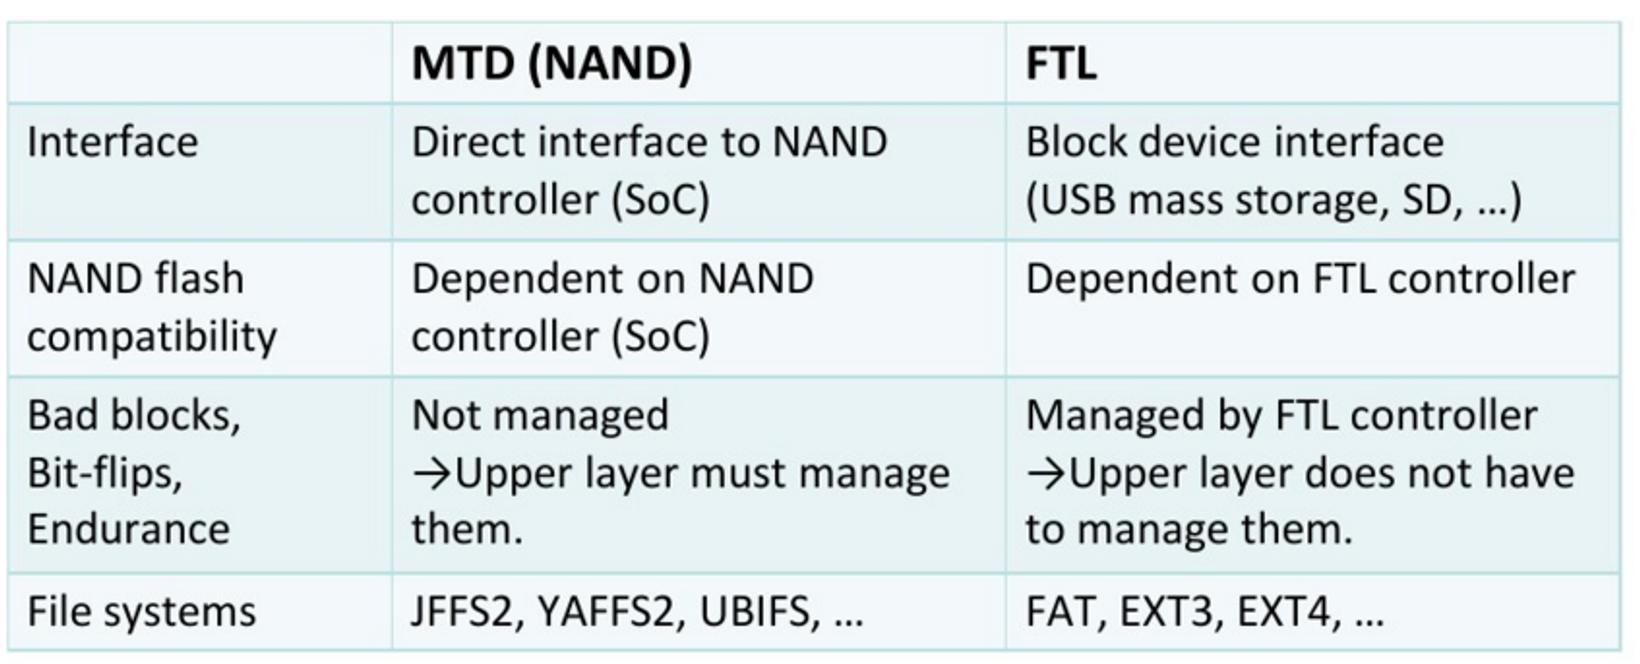
\includegraphics[width=0.7\textwidth]{fig/flash-mtd-ftl}
  \caption{MTD 设备和有 FTL 的设备的对比}
  \label{flash-mtd-ftl}
\end{figure}

MTD 设备和有 FTL 的设备的对比如图 \ref{flash-mtd-ftl} 所示。在我们的项目中,我们选择了基于 Nand Flash 的块设备,而不是基于 Nand Flash 的 MTD 设备,这样可以更加贴近实际应用场景,扩展项目的实际用途,也可以更加容易地和其他的文件系统进行对比。

我们选择基于 Nand Flash 与 FTL 的文件系统,题目需求中的许多方面都出现了新的需求。首先,Nand Flash 的读写单位是页,而 Nor Flash 的读写单位是字节,这就要求我们的文件系统在读写时要考虑到页的边界对齐问题。其次,Nand Flash 之上的一层 FTL,向上隔绝了数据块选择、数据擦除、逻辑物理地址映射等与 Flash 存储介质相关的细节,从而提高了在文件系统层面针对 Flash 进行优化的难度。最后,Nand Flash 的读写速度比 Nor Flash 快,但是擦除速度比 Nor Flash 慢,这就要求我们的文件系统在设计时要考虑到这一点,尽量减少擦除操作的次数。

为了解决这些问题,我们需要对 Nand Flash 的特性进行调研,然后在一种基于 Nand Flash 的文件系统的基础上进行改进。

\subsection{背景调研}

在我们选定赛题后,我们立刻开始了针对 Flash 文件系统实现的调研。

\subsubsection{Flash 的特点和分类}

为了实现针对 Flash 优化的文件系统,我们必须首先了解 Flash 的各种特性和分类。

闪存(Flash Memory)是由日本的 舛岡富士雄 (Fujio Muoka)发明的。他分别于1966年和1971年从日本东北大学(Tohoku University)获得学士和博士学位,博士毕业之后他加入了东芝(Toshiba)公司。在东芝工作期间,他分别于1980年和1988年发明了NOR Flash 和 Nand Flash。

目前市面上的闪存主要有两种:NOR Flash 和 Nand Flash,其分类逻辑和原理如图 \ref {flash-nand-nor} 所示。
一般而言,并行接口的Parallel Flash是基于NOR Flash的;而SSD硬盘,U盘,SD卡,eMMC等通常是基于Nand Flash的。

\begin{figure}[htbp]
  \centering
  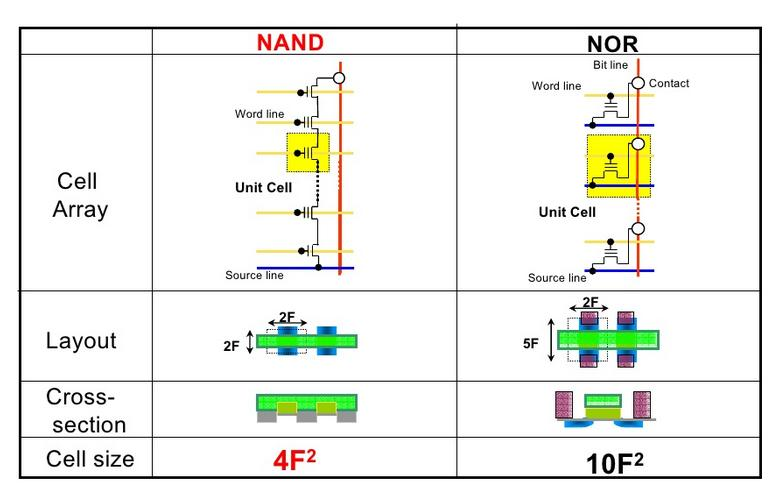
\includegraphics[width=0.85\textwidth]{fig/flash-nand-nor}
  \caption{Flash 原理与分类}
  \label{flash-nand-nor}
\end{figure}

\subsubsection{Nand Flash}

Nand Flash 是一种非易失性存储器,具有访问速度快、存储密度高、成本低的特点。Nand Flash 的读写操作都是以页为单位进行的,而且每次写操作都需要先擦除整个块,这使得 Nand Flash 更适合用于存储大量数据,而不适合用于执行代码和固件更新等应用。然而,Nand Flash 的读写速度快,成本低,是目前大多数嵌入式设备或消费级、商业级电子产品的主要存储介质。

\begin{figure}[htbp]
  \centering
  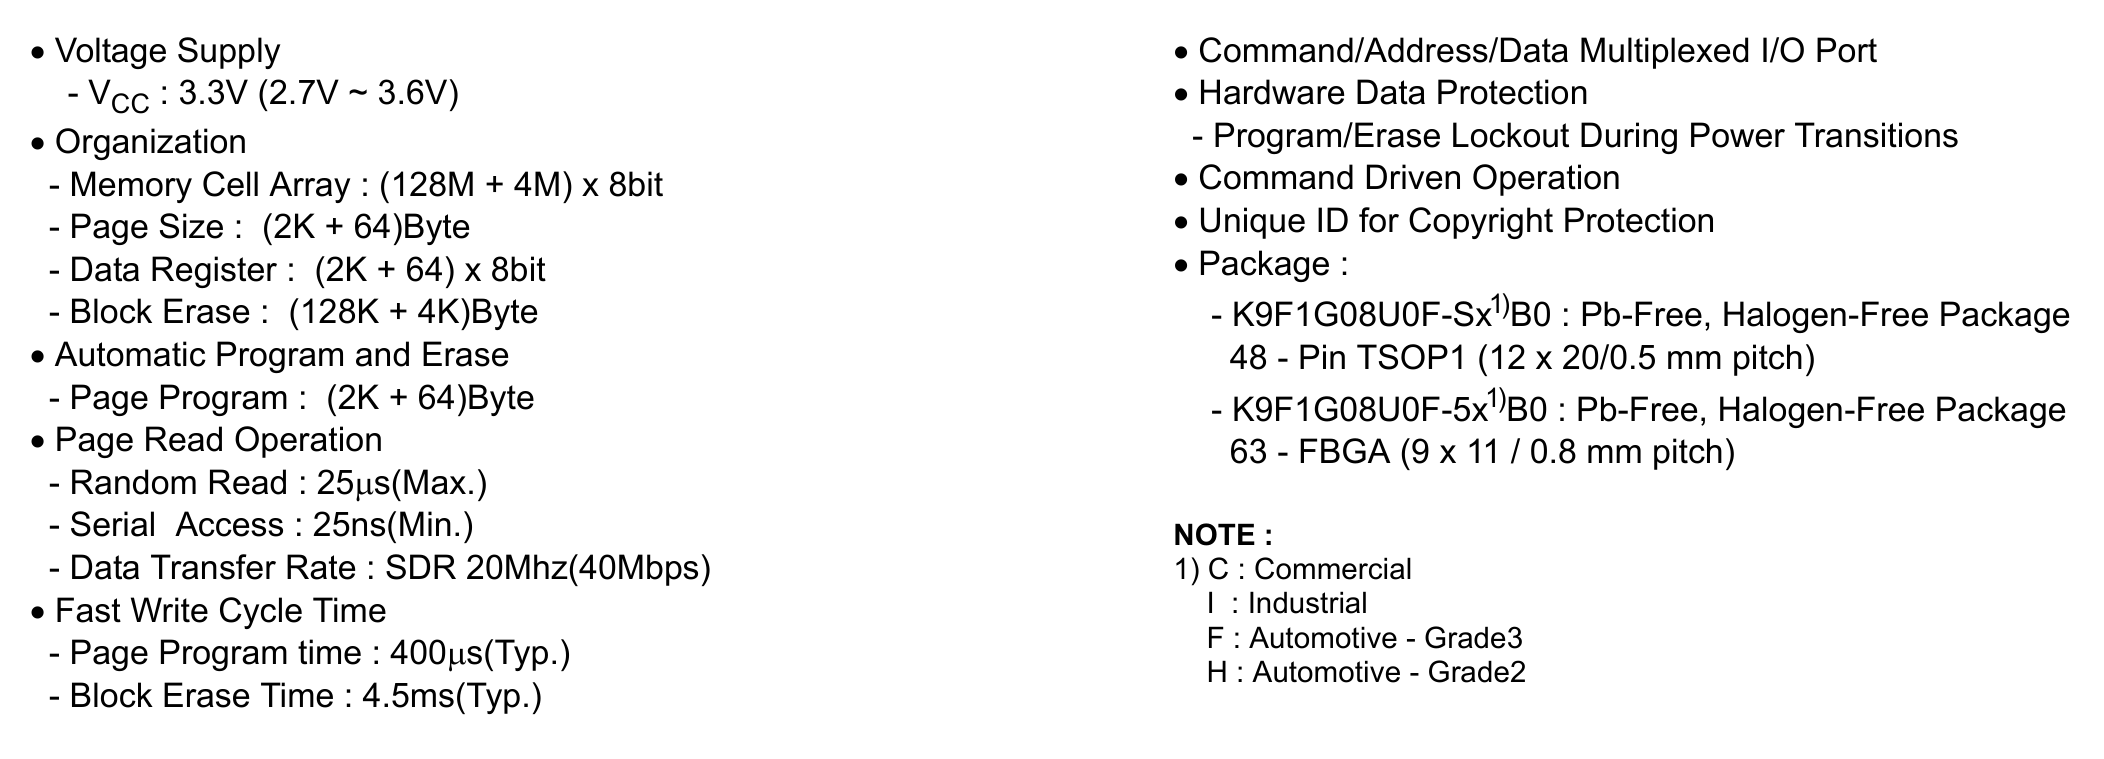
\includegraphics[width=0.85\textwidth]{fig/flash-nand-feature}
  \caption{K9F1G08U0F-5IB0 特性}
  \label{flash-nand-feature}
\end{figure}

为了详细了解 Nand Flash 的多种特性,我们专门针对一款常用的 Nand Flash 进行了调研。这款 Nand Flash 的型号是 K9F1G08U0F-5IB0。这是一款来自三星的 SLC Nand,容量为 1Gb,其主要特性如图 \ref{flash-nand-feature} 所示。

在读写操作失败时,Nand 控制器需要进行一些特殊的处理。将 Datasheet 中的处理方式翻译为中文:在 NAND Flash 存储器中,其使用寿命内可能会出现额外的无效块。请参考资格报告以获取实际数据。应考虑以下可能的故障模式以实现高度可靠的系统。在擦除或编程后状态读取失败的情况下,应进行块替换。因为在页面编程期间的编程状态失败不会影响同一块中其他页面的数据,所以可以通过找到一个已擦除的空块,并重新编程当前目标数据并复制替换块的其余部分,来执行块替换。在读取时必须使用 ECC。为了提高内存空间的效率,建议通过 ECC 回收由于单个位错误而导致的读取或验证失败,而无需进行任何块替换。所述附加块故障率不包括那些被回收的块。写入时错误处理流程如图 \ref{nand-rw-err} 所示。

\begin{figure}[htbp]
  \centering
  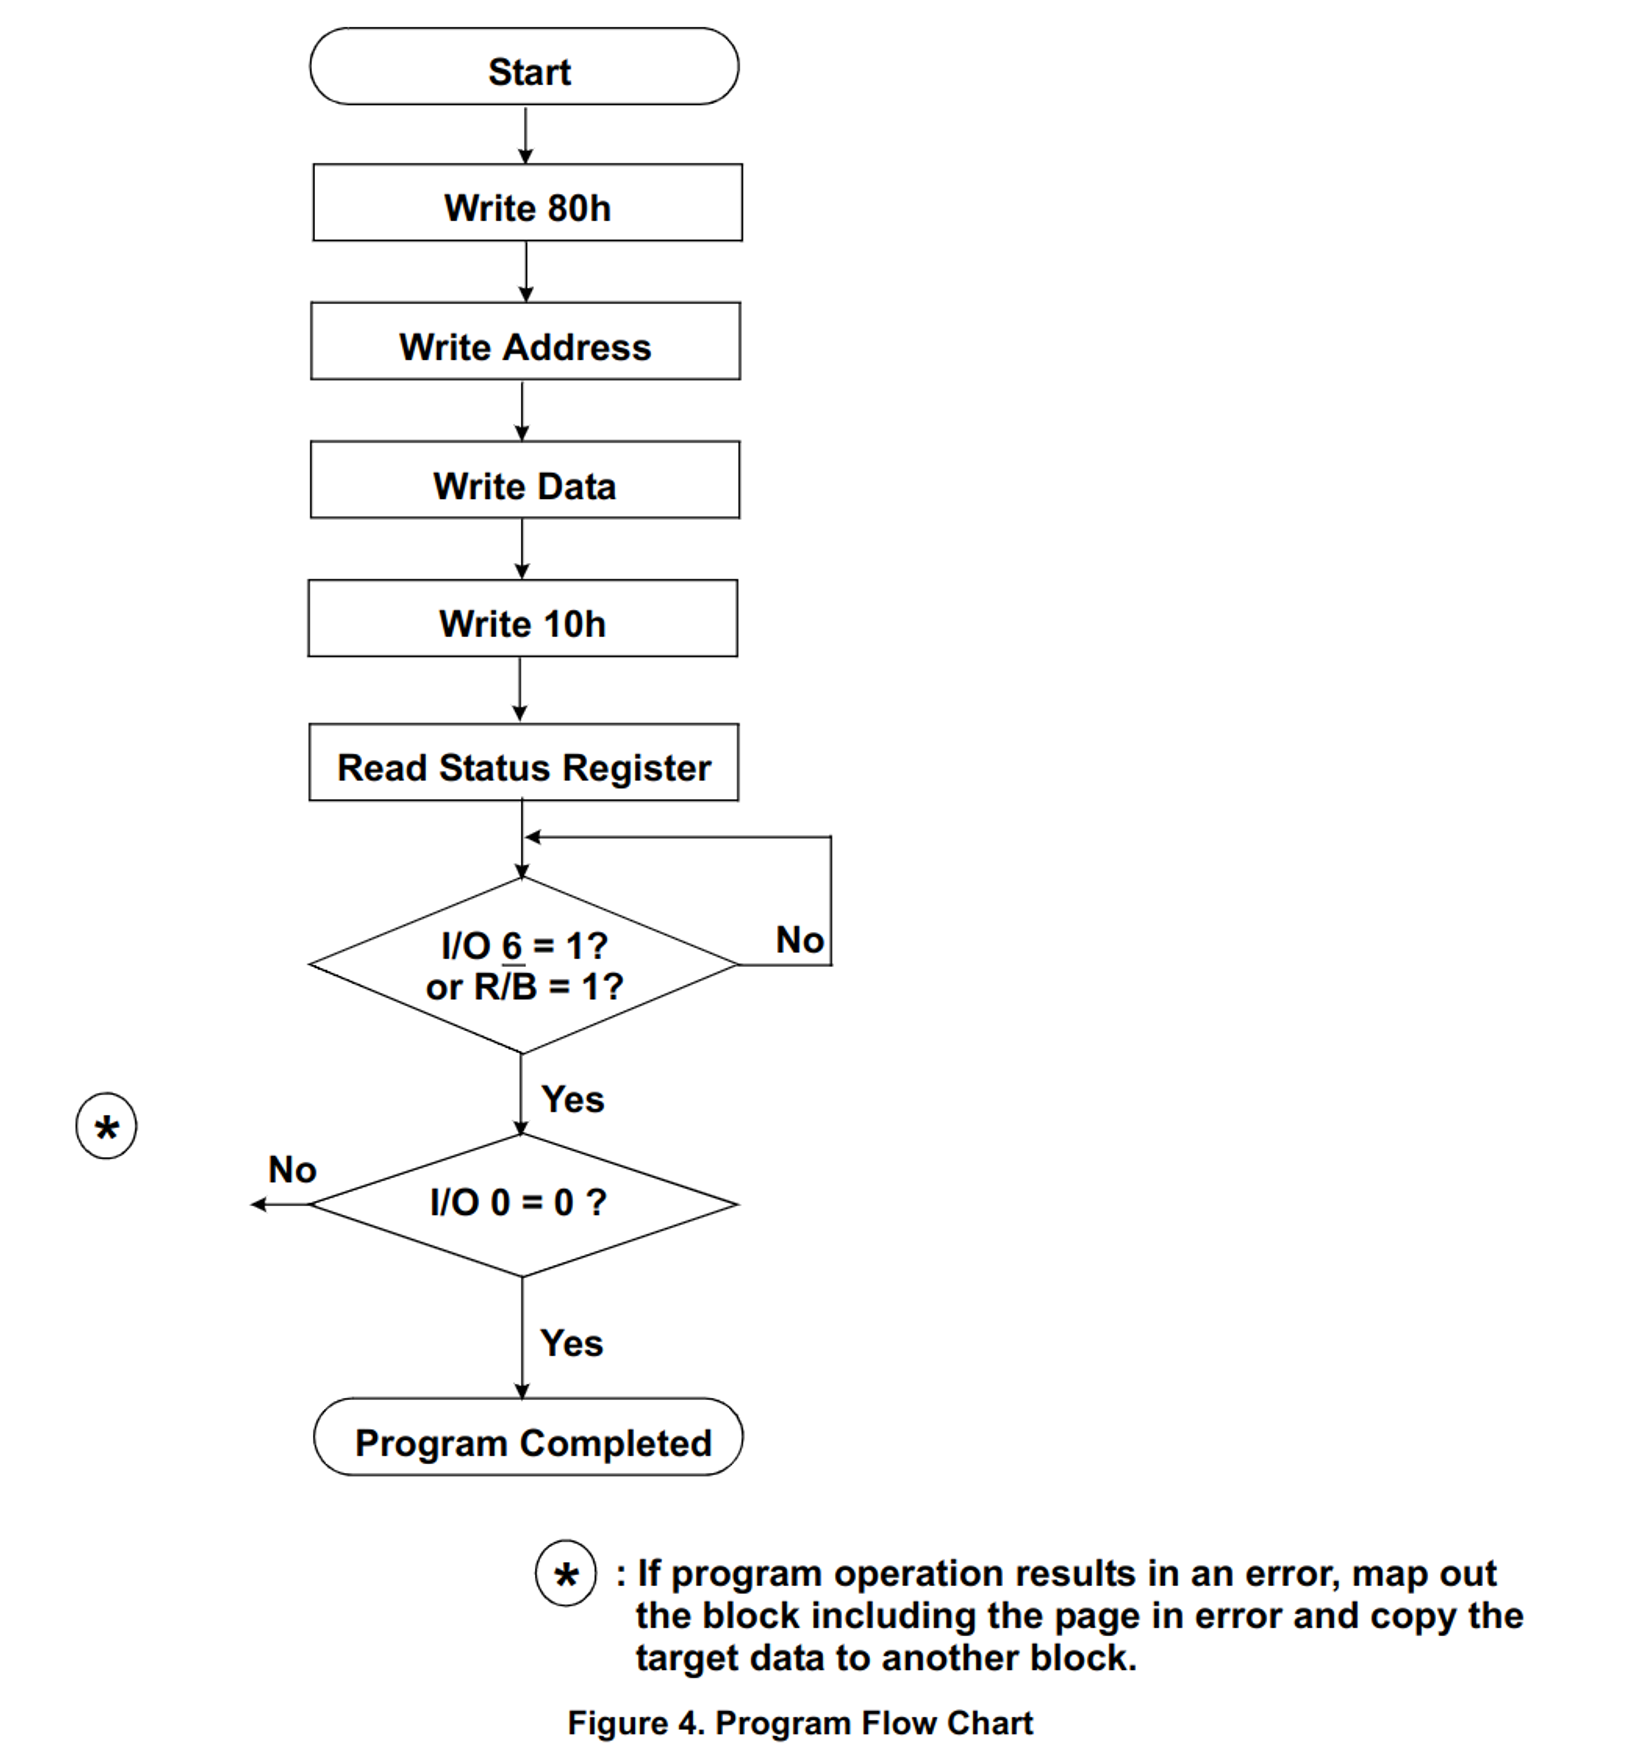
\includegraphics[width=0.85\textwidth]{fig/nand-rw-err}
  \caption{写入时错误处理流程}
  \label{nand-rw-err}
\end{figure}

Nand 由于其以页面为写入单位的特性,使得其在写入时的错误处理流程较为复杂。在写入时,如果发生错误,需要进行块替换。块替换的过程如图 \ref{nand-replace} 所示。

\begin{figure}[htbp]
  \centering
  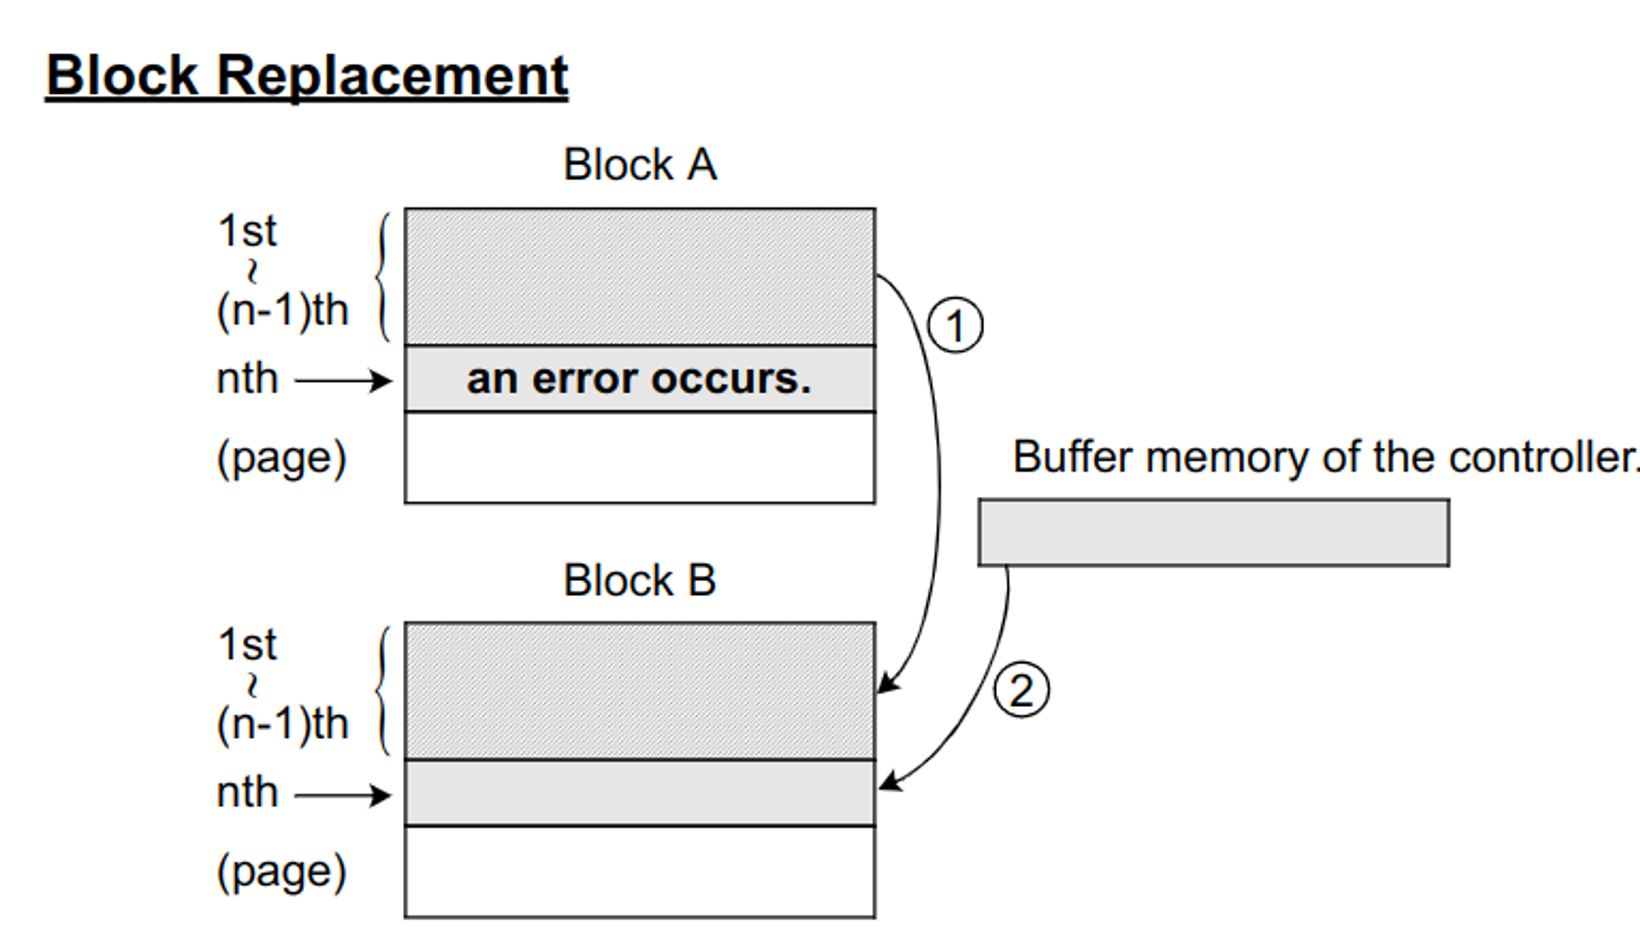
\includegraphics[width=0.85\textwidth]{fig/nand-replace}
  \caption{Nand 块替换流程}
  \label{nand-replace}
\end{figure}

由于 Nand Flash 只能以页面为单位进行写入,所以在一个块内,页面必须从该块的LSB(最低有效位)页面到该块的MSB(最高有效位)页面依次编程,禁止随机页面地址编程。在这种情况下,LSB页面的定义是要编程的页面中的LSB。因此,LSB不需要是页面0。

\begin{figure}[htbp]
  \centering
  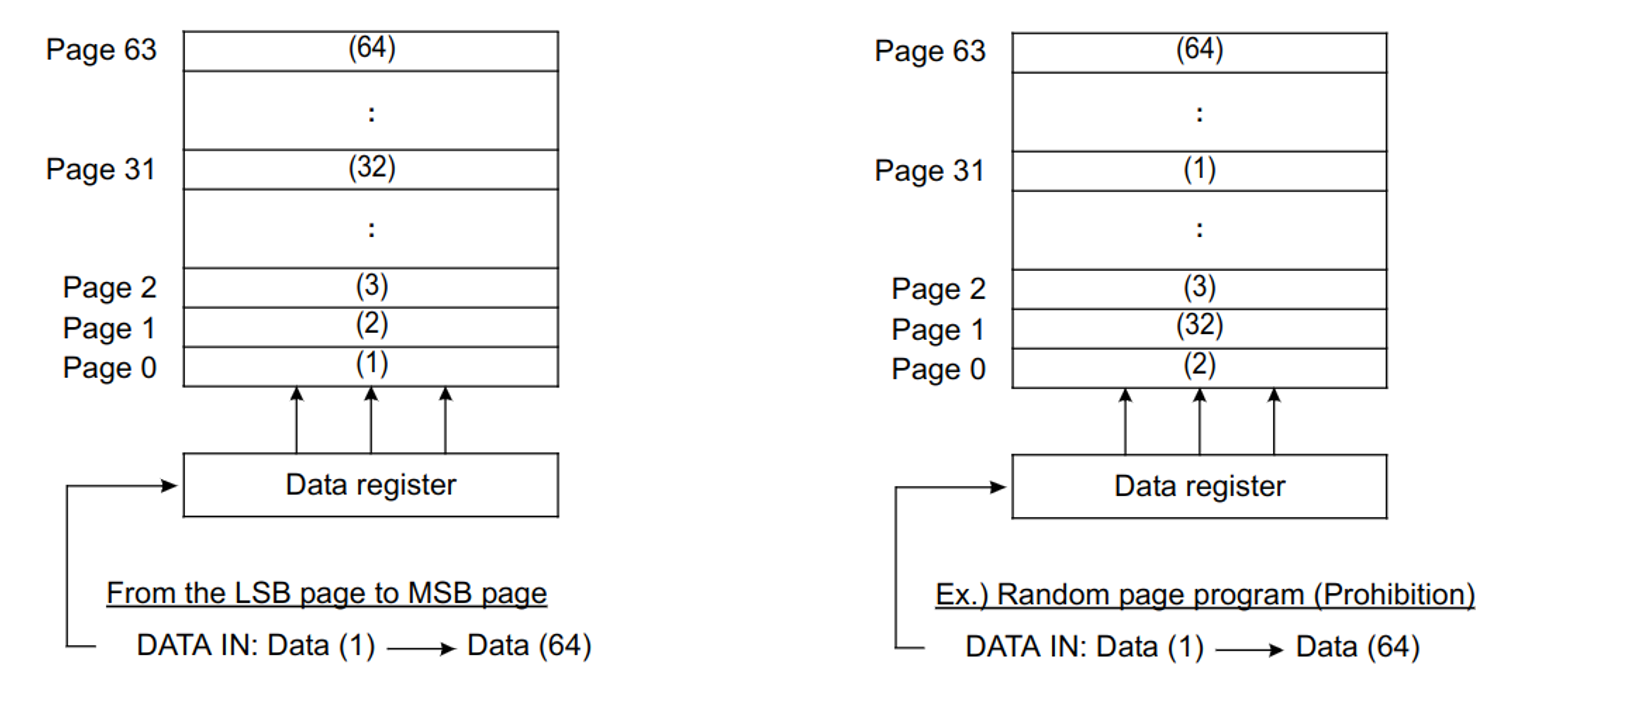
\includegraphics[width=0.85\textwidth]{fig/nand-write-addr}
  \caption{Nand 写入寻址举例}
  \label{nand-write-addr}
\end{figure}

这个用于举例的 Flash 芯片已带有 ECC 功能。在编程操作期间,内部ECC逻辑生成ECC。在读取操作期间,设备会自动执行ECC。读取操作执行后,可以发出读取状态命令以识别读取状态,读取状态保持不变,直到执行其他有效命令。这个 Nand Flash 可以自己纠正 4bit 的错误。

即,这款 Nand 芯片内的控制器能够保证在读取时,能够自动执行 ECC,并且能够自动纠正 4bit 的错误。这样,我们在读取时,基本不需要考虑较少比特位的 ECC 的问题。当 Nand 芯片内的控制器检测到无法纠正的 ECC 错误,将会返回错误信息,然后可以根据这个错误信息,进行块替换。如果块替换失败,那么这个块就会被标记为坏块,不再使用。

由此得知,一般 Nand 芯片向外提供的数据接口可以保证数据的正确性,从而上层软硬件可以依赖于 Nand 上的硬件 ECC 提供的数据正确性保证。但是这是在 Nand 使能了 ECC 功能的情况下,如果 Nand 芯片没有使能 ECC 功能,那么上层软硬件就需要自己实现 ECC 算法,来保证数据的正确性。此外,硬件 ECC 功能需要占用额外的磁盘空间,因此,如果对磁盘空间有较高要求,那么可以考虑不使能硬件 ECC 功能。

\subsubsection{Nor Flash}

NorFlash 是一种非易失性存储器,具有访问速度快、读写寿命长、可靠性高的特点。与 Nand Flash 不同,NorFlash 的读操作可以以随机方式进行,而不需要预先擦除整个块。这使得 NorFlash 更适合用于执行代码和固件更新等应用,可以加速启动时间和提高系统性能。然而,NorFlash 的密度较低,成本较高,不适合用于存储大量数据。

NorFlash 的一些其他特点包括:

\begin{itemize}
  \item {\bf{高度可靠}}:Nor Flash 可以实现数据的可靠存储和读取,并且具有高度可靠性。
  \item {\bf{可以执行代码}}:Nor Flash 可以作为代码存储器,可以加快启动时间并提高系统性能。此外,Nor Flash 还支持 XIP(执行内存),它允许 CPU 直接从 Nor Flash 中执行代码,而无需将代码加载到 RAM 中。
  \item {\bf{读写寿命}}:Nor Flash 的读写寿命比 Nand Flash 长得多,因此它更适合于需要高度可靠性和长寿命的应用程序。
  \item {\bf{错误概率}}:Nor Flash 读写操作的错误概率很低,这使得它在数据存储和传输方面更加可靠。
\end{itemize}

\subsubsection*{Nand flash 和 Nor flash 的性能比较}

flash闪存是非易失存储器,可以对称为块的存储器单元块进行擦写和再编程。任何flash器件的写入操作只能在空或已擦除的单元内进行,所以大多数情况下,在进行写入操作之前必须先执行擦除。NAND器件执行擦除操作是十分简单的,而NOR则要求在进行擦除前先要将目标块内所有的位都写为0。由于擦除NOR器件时是以64~128KB的块进行的,执行一个写入/擦除操作的时间为5s,与此相反,擦除NAND器件是以8~32KB的块进行的,执行相同的操作最多只需要4ms。执行擦除时块尺寸的不同进一步拉大了NOR和NADN之间的性能差距,统计表明,对于给定的一套写入操作(尤其是更新小文件时),更多的擦除操作必须在基于NOR的单元中进行。

Nand Flash 与 Nor Flash 的主要区别如下:

\begin{itemize}
  \item NOR的读速度比NAND稍快一些。
  \item NAND的写入速度比NOR快很多。
  \item NAND的4ms擦除速度远比NOR的5s快。
  \item 大多数写入操作需要先进行擦除操作。
  \item NAND的擦除单元更小,相应的擦除电路更少。
\end{itemize}

我们最终选定了 Nand Flash 作为我们的存储介质,主要是因为 Nand Flash 的价格更低,而且 Nand Flash 的读写速度更快,更适合于我们的应用场景,同时与其他赛组的工作能保持一定的区分度。

\subsubsection{FTL}

FTL(Flash Translation Layer,闪存地址翻译层)是广泛存在于 Nand Flash 存储层次之上的一层地址翻译逻辑,它的主要作用是将逻辑地址转换为物理地址。

FTL 通常是由 Nand Flash 的厂商提供的,因此,不同厂商的 FTL 实现可能会有所不同,但是它们的主要功能都是相同的,即地址映射。原因是闪存只能异地更新,为了对上支持数据块原地更新则需要通过地址转换实现。由于闪存先擦后写、擦写有次数限制(寿命)、使用过程中会不断出现坏块(块寿命不同)等特性,FTL还需具备垃圾回收、磨损均衡、坏块管理等十八般武艺。

闪存内部的基本存储单位是Page(4KB),N个Page组成一个Block。FTL 的映射方式主要有:

\begin{enumerate}

  \item \textbf{块级映射}

  将块映射地址分为两部分:块地址和块内偏移。映射表只保存块的映射关系,块内偏移直接对应。

  \item \textbf{页级映射}

  映射表维护每个页的映射关系。

  \item \textbf{混合映射}

  主要思路是针对频繁更新的数据采用页级映射,很少更新的数据采用块级映射。其中采用Log Structured思想的混合映射将存储分为数据块(Data Block)和日志块(Log Block)。数据块用于存储数据,采用块级映射,日志块用于存储对于数据块更新后的数据,采用页级映射。混合映射是低端SSD、eMMC、UFS广泛采用的映射方式。根据日志块和数据块的对应关系又可以分为全相关映射(FAST)、块相关映射(BAST)、组相关映射(SAST)等等。下图是SAST映射的一个示例:2个日志块对应4个数据块,当日志块用完时需要通过搬移有效数据回收日志块。对于顺序写场景,最好情况下日志块对应位置记录了数据块的更新,则可以无需搬移数据,直接将日志块作为新的数据块,数据块进行擦除操作作为新的日志块。对于大量随机写场景,则需要将日志块和数据块中的有效数据搬移到空闲块的对应位置作为新的数据块,然后擦除原日志块和数据块。

\end{enumerate}

由于 FTL 一般实现在 SSD/EMMC 主控中,作为一个黑盒存在,因此上层软件无法得知 FTL 的具体实现,也无法对其进行优化。举个例子,如果上层软件知道 FTL 的映射方式是页级映射,那么它就可以将多个小文件合并成一个大文件,这样就可以减少 FTL 的映射表的大小,从而提高性能。但是上层软件往往并不知道 FTL 的映射级别和映射表的大小,因此无法进行优化;如果软件贸然进行优化,反而可能会触发 FTL 的垃圾回收机制等,从而造成更大的写放大和性能降低。

此外,FTL 的映射逻辑需要占用一定的存储空间,这也是 FTL 的一个缺点。加上主控的垃圾回收功能,一款 SSD 往往有 10\% 到 20\% 的空间是不可用的,这也是 SSD 的一个缺点。

\subsubsection{SSD 的性能瓶颈}

SSD 的性能瓶颈涉及多个方面:

首先,闪存芯片本身的读取和写入速度是一个重要的性能瓶颈。尽管闪存技术不断进步,但相对于传统的机械硬盘,闪存的读取和写入速度仍然有限。特别是对于随机的小块读写操作,闪存的延迟和响应时间可能较高。

其次,闪存芯片的擦写操作是一项耗时的操作,因为擦除一个块通常需要先将其数据复制到其他位置,然后进行擦除操作。这导致了写入操作的额外开销和延迟,尤其在频繁的写入场景下,擦写操作的成本会进一步增加。

另外,闪存芯片的寿命限制也是一个性能瓶颈。闪存芯片具有有限的擦写次数,每次擦写操作都会减少芯片的寿命。当某些块的擦写次数达到上限时,需要进行垃圾回收和数据迁移操作,这可能导致额外的延迟和性能损耗。

存储控制器也对SSD的性能起着重要作用。存储控制器负责管理闪存芯片、处理IO请求、执行错误校验和纠正(ECC)等功能。较低性能的存储控制器可能成为整个系统的瓶颈,限制了SSD的性能表现。

最后,接口和总线的带宽限制也可能影响SSD的性能。常见的接口如SATA、PCIe、NVME等,其带宽和传输速度对于数据的读取和写入速度有一定影响。如果接口和总线的带宽无法满足SSD的性能要求,可能会限制SSD的吞吐量和响应时间。

我们选定了需要做基于 Nand Flash 的文件系统,就必须要直面以上的问题,我们需要在文件系统层面上解决这些问题,使得文件系统能够更好的利用 Nand Flash 的特性,提高文件系统的性能。

经过调研,我们发现了许多现有的基于 Nand Flash 的文件系统,如 Btrfs、LogFS、F2FS 等。这些文件系统都是为了解决 Nand Flash 的特性而设计的,它们都有各自的优缺点,但是都是在当下已经有完善的 FTL 映射的情况下去解决这个问题。

如果有一种“文件系统”,能够在上层软件和下层硬件之间沟通协调,让软硬件各自更加各司其职,做更适合做的事情,那么能不能解决上面提到的诸多困难呢?

于是乎,我们找到了 ZenFS。这是一个简单的“文件系统”,但是它却能够做到保持最高性能写入不掉速,能做到 100\% 的空间利用率,能做到最高的数据库随机读写速度和最低的读写延迟。对这样一种“文件系统”,我们立刻产生了极大的兴趣。对 ZenFS 的调研,详见第 \ref{chap:zenfs} 章的介绍。

\subsubsection{文件系统调参}

在数据库和文件系统这些存储系统中中实现良好的性能并非易事,因为它们是复杂的系统,具有许多可调选项,这些选项几乎控制其运行时操作的许多方面。在这些系统中,配置参数是一个重要的问题。存储系统通常有许多影响其行为的参数,调整这些参数可以显着提高性能。由于大量的参数和可能的配置呈指数级增长,手动和自动调整方法都很费力。

鉴于此,许多组织会聘请昂贵的专家来配置系统的参数。但是随着应用程序在规模和复杂性方面的增长,优化参数以满足应用程序的需求已经超越了人类的能力。这是因为参数的正确配置在很大程度上取决于许多人所无法推理的因素。

于是,我们预期实现一个智能调参模块来使得作为RocksDB插件的文件系统AquaFS具有自动调整本身参数的能力,以使得文件系统更加智能,减少可能的人力开销。

在智能调参方面主要设计到两个方面,参数选择和参数调整。

在参数选择方面,存储系统通常有许多影响其行为的参数。存储系统是现代计算机系统的关键组件,对应用程序性能和效率有重大影响。大多数存储系统都有许多可配置的参数来控制和影响它们的整体行为。例如,Linux 的Ext4提供了大约60个参数[1],代表超过 1037种潜在的配置状态。默认设置通常不是最优的;有研究表明,调整存储参数可以将系统性能提高多达 9倍[2]。

为了应对大量可能的配置,系统管理员通常专注于使用他们的领域专业知识来调整一些经常使用和经过充分研究的参数,这些参数被认为会显着影响系统性能。然而,面对日益增加的复杂性,这种手动调整方法并不能很好地扩展。现代存储系统使用不同的文件系统类型(EXT4,XFS,Btrfs)、新硬件(SSD、SMR、NVM)、多层和混合存储,和多个虚拟化层(例如 LVM、RAID)。存储系统范围从一个或几个相同的节点到数百个高度异构的节点在参数调整方面。

最近,已存在多种优化方法来自动调整存储系统,在合理的时间范围内实现了良好的性能改进 [3,4]。这些自动调整技术将存储系统建模为黑匣子,反复尝试不同的配置,测量目标函数的值,并根据先前学习的信息选择新的配置进行尝试。然而,许多黑盒自动调整技术难以扩展到高维,并且可能需要很长时间才能收敛到好的解决方案。因此,处理大量存储参数配置的问题在很大程度上仍未解决。

在机器学习和信息论中,降维是处理大型数据集的常用技术。如果它可以应用于存储系统,它将大大减少搜索空间,使人类或算法更容易调整存储系统。以前的研究中提到,并非所有存储参数都具有同样重要的性能影响:一些参数比其他参数具有更大的影响 [3]。这自然促使我们研究如何量化每个存储参数的影响或重要性,以及如何有效地选择重要参数。

现在存在许多方法来解决维数灾难的问题,也即降维方法。降维方法通常可以概括为两类:特征提取和特征选择。

特征提取是指将高维数据投影到低维空间;新构建的特征通常是原始特征的线性或非线性组合。常见的特征提取方法包括主成分分析 (PCA)、独立成分分析和线性判别分析。特征提取的一个主要缺点是每个特征的物理意义都会因投影和许多维度的非线性组合而丢失。因此,常见的特征提取技术与本文中的目标相冲突:即选择一些可以理解和解释的原始存储参数。

相反,特征选择直接从原始特征中选择一个特征子集,目的是只找到重要的特征。特征选择方法可以分为监督或非监督方法。无监督特征选择,例如 Principle Feature Analysis ,根据特征之间的关系选择包含大部分基本信息的子集。在选择阶段不考虑特征对优化目标的影响。相反,有监督的特征选择选择一个可以区分或近似目标变量的子集。其中包括基于决策树的算法等等。由于我们有兴趣找到对我们的优化目标有重大影响的参数,例如 I/O 吞吐量,因此监督特征选择最适合我们的需求。

由于在存储系统中存在许多离散的参数,将这些离散参数抽象成离散值的质量决定了特征选择的质量,将具有 N 个值的分类参数转换为 N 个单独的二进制参数会使参数空间呈指数级扩展。因此本文并没有采用lasso回归,lasso回归的计算成本很高。

另一种流行的特征选择方法是建立在信息论的基础上的方法。这些方法通常为某些子集中目标变量的同质性定义一个度量。常用的指标包括连续变量的方差等。在本文中,们采用基于方差的重要参数选择方案,方差在系统中的对比可以凸显出参数的重要性。

在参数调整方面,是对于参数选择中的重要参数进行参数的调整。

在之前的对数据库进行自动调参的研究中[6],对数据库的表征负载进行提取,在匹配了相似负载,并用lasso回归对参数进行去冗余降维之后,采用了高斯过程回归的方案进行参数的调整。高斯过程回归是一种先进的技术,其功能与深度网络的功能大致相当。高斯过程回归有许多吸引人的特性,使其成为配置空间建模和提出建议的合适选择。最重要的是,一个是高斯过程回归默认提供置信区间。在该研究中采用了两种方案提供推荐的参数,其中一种是直接匹配相似负载中的最好配置,另外一种是尝试回归的配置。本文中尝试使用两种方案。

\subsection{ZenFS}
\label{chap:zenfs}

\subsubsection{ZenFS 的特点}

ZenFS 是一个 RocksDB 的文件系统插件,它利用 RocksDB 的文件系统接口将文件放置到原始分区块设备上的区域中。通过将文件分成多个区域并利用写入生命周期提示来共同定位具有相似生命周期的数据,与传统的块设备相比,系统写入放大大大降低了。 ZenFS 确保文件系统或磁盘上没有后台垃圾收集,从而提高吞吐量、尾部延迟和磁盘耐久性方面的性能(图 \ref{zns-write})。ZenFS 的整体架构如图 \ref{zenfs-overview} 所示。

\begin{figure}[htbp]
    \centering
    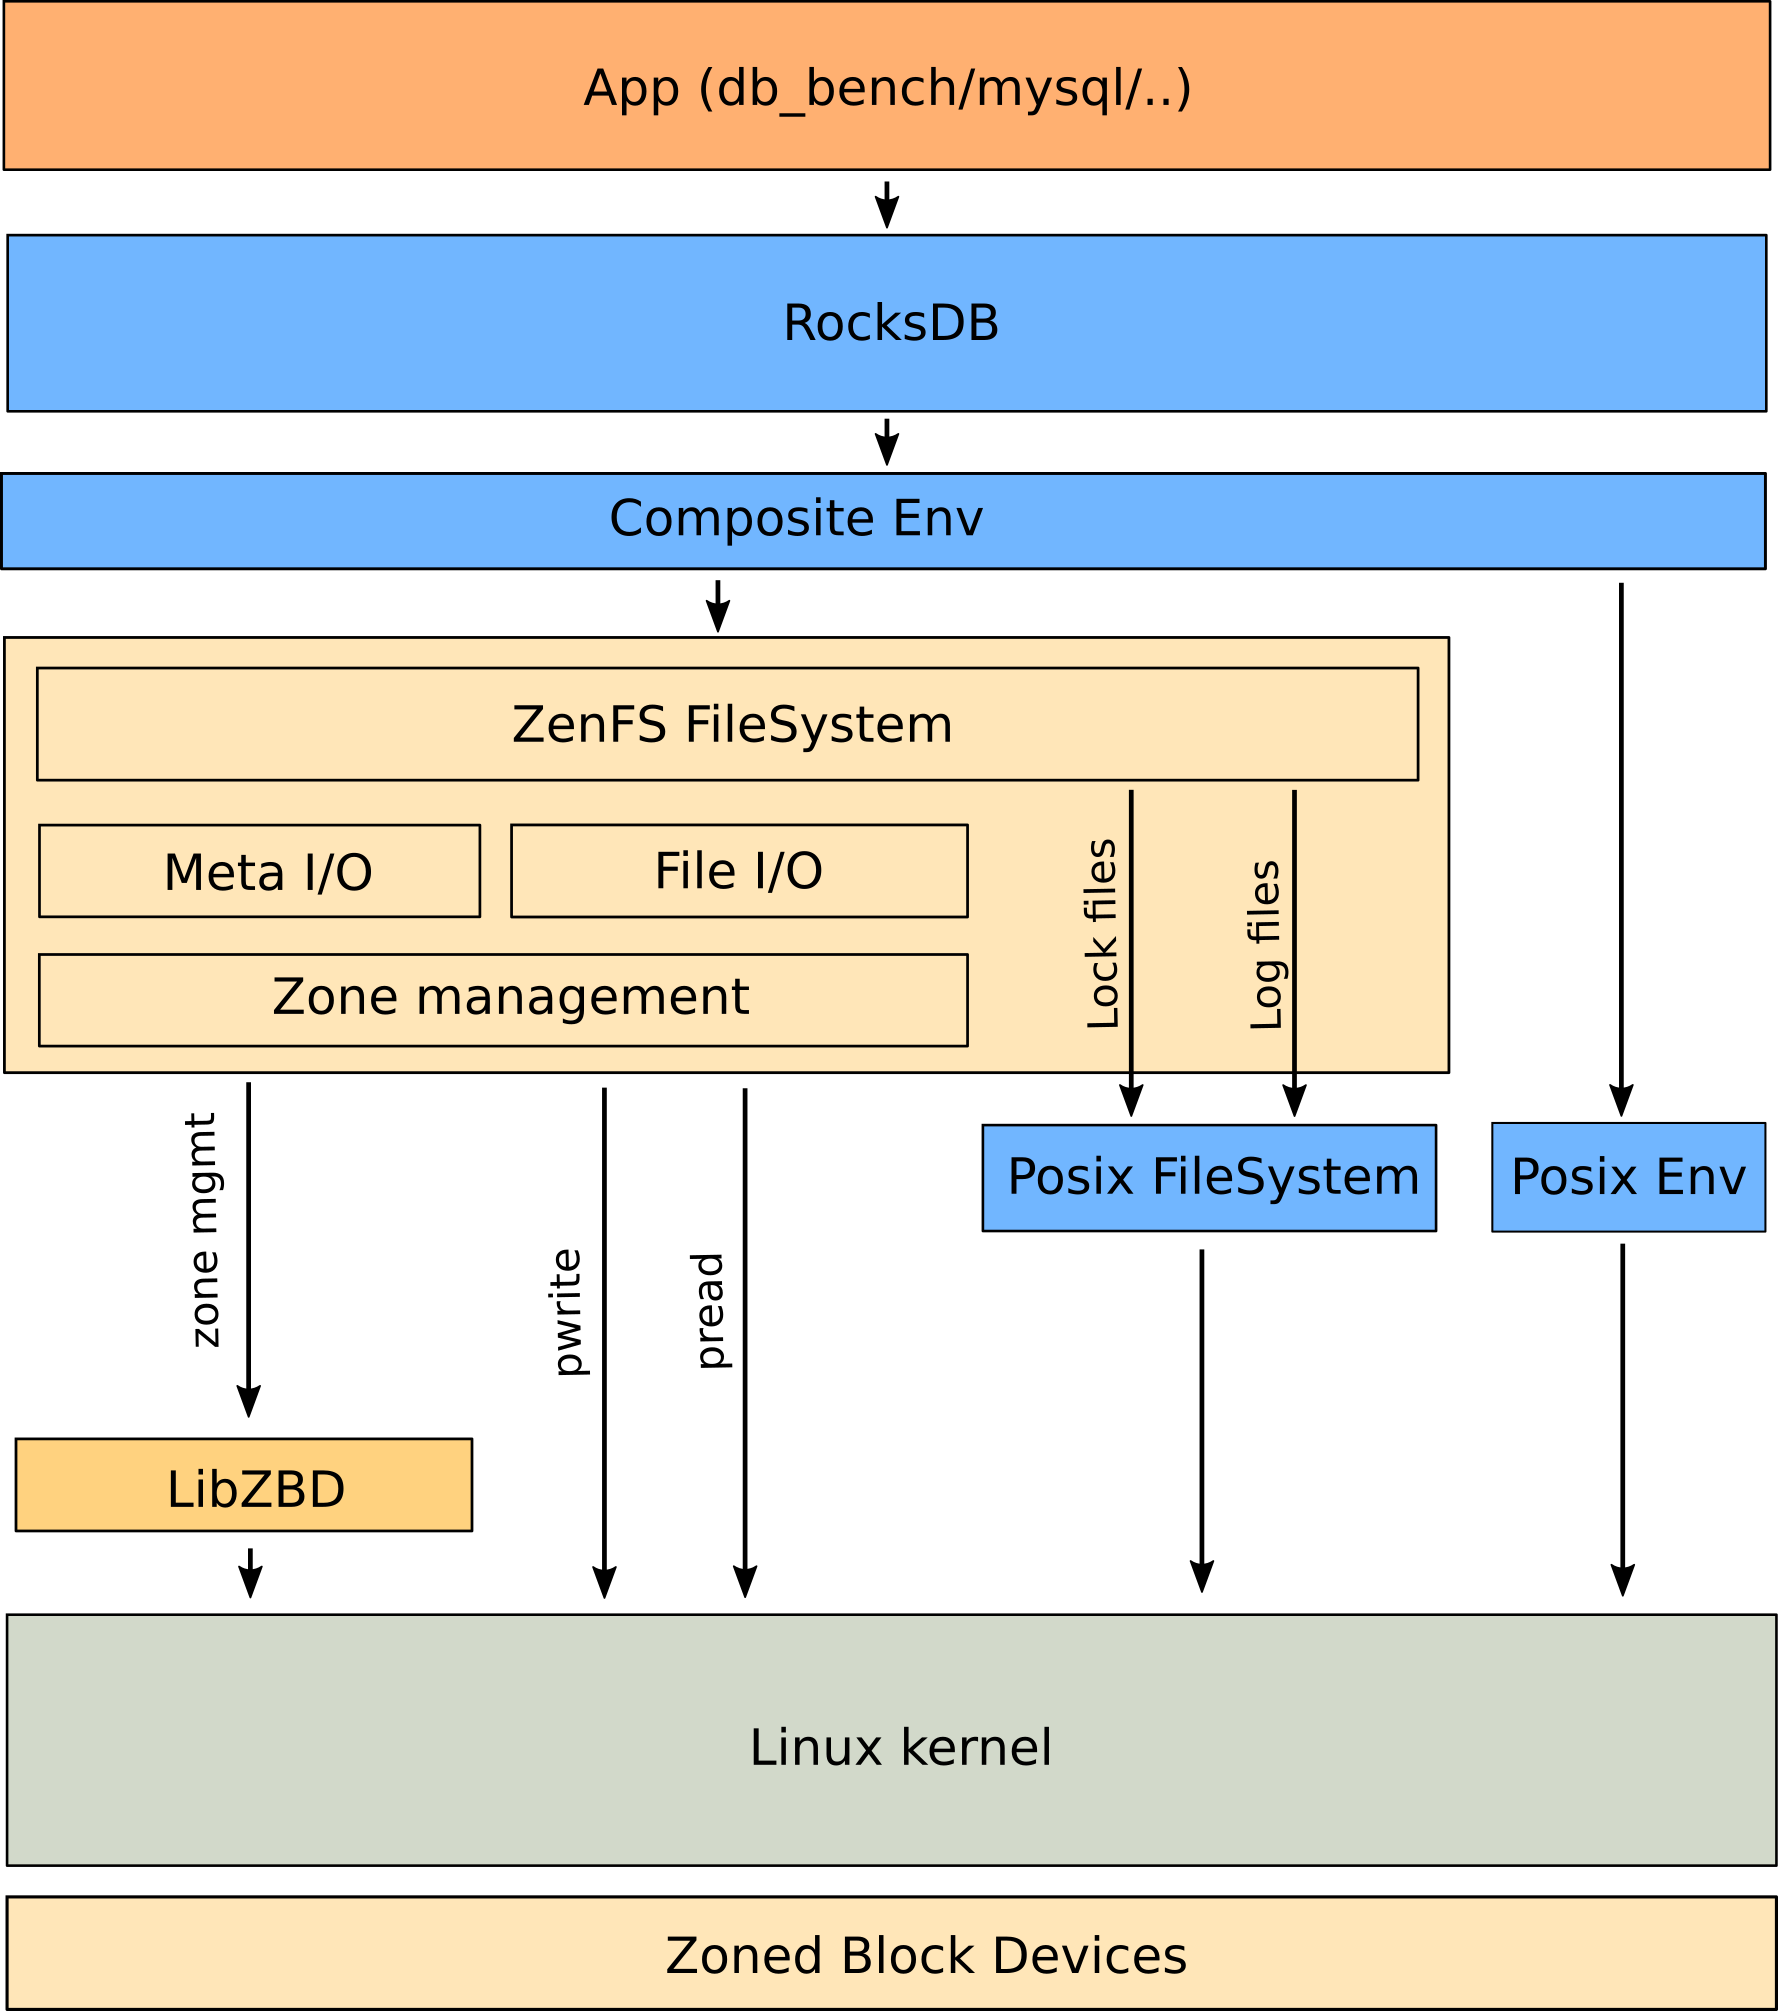
\includegraphics[width=0.8\textwidth]{fig/zenfs-overview}
    \caption{ZenFS 架构}
    \label{zenfs-overview}
\end{figure}

\begin{figure}[htbp]
    \centering
    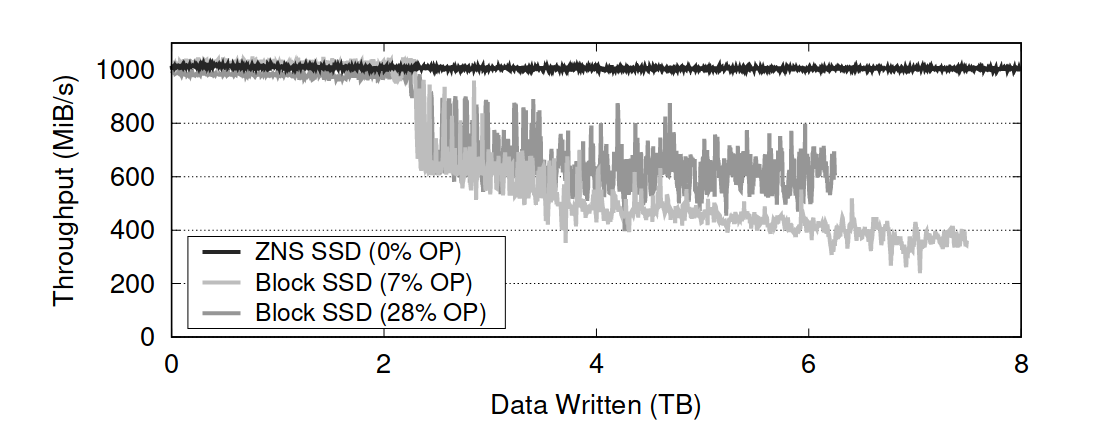
\includegraphics[width=0.8\textwidth]{fig/zns-write}
    \caption{ZNS 多线程完全覆盖写入负载下吞吐量表现}
    \label{zns-write}
\end{figure}

ZenFS 是一种特殊的“文件系统”。与其说是一种文件系统,不如说是一种全新的软硬件协同的系统中的一部分。它通过尽量将原本不可知的 FTL 映射和垃圾回收的过程暴露给上层,使得上层可以更好地利用 SSD 的特性。ZenFS 通过将文件分成多个区域并利用写入生命周期提示来共同定位具有相似生命周期的数据,与传统的块设备相比,系统写入放大大大降低了。ZenFS 确保文件系统或磁盘上没有后台垃圾收集,从而提高吞吐量、尾部延迟和磁盘耐久性方面的性能。

硬件方面,ZenFS 基于 Zoned Storage SSD 和 ZNS(Zoned Namespaces)。

ZNS 是 NVMe 最新标准的一部分,它是专用于特殊 SSD 的通用接口,能够将更多的信息暴露到主机上,利用主机的应用场景信息来优化 SSD 的性能。而 Zoned Storage SSD 就是专门为 ZNS 而设计的 SSD,它将 SSD 的内部划分为多个区域,每个区域都有自己的写入指针,不支持随机写入而是只支持从当前写指针写入,从而尽可能地避免了底层主控上的逻辑映射和垃圾回收。普通 SSD 的主控掌握了逻辑地址到物理地址的映射,并且在主机不可控的情况下执行垃圾回收(尽管有 Trim 命令的支持),而 Zoned Storage SSD 的垃圾回收机制是由主机来控制的,这样就可以最大程度上地减小写入放大和读写波动,并且能够完全消除硬件预留的空间,从而提高了 SSD 的性能利用率。Zones 的地址空间和写逻辑如图 \ref{zns} 所示。

\begin{figure}[htbp]
    \centering
    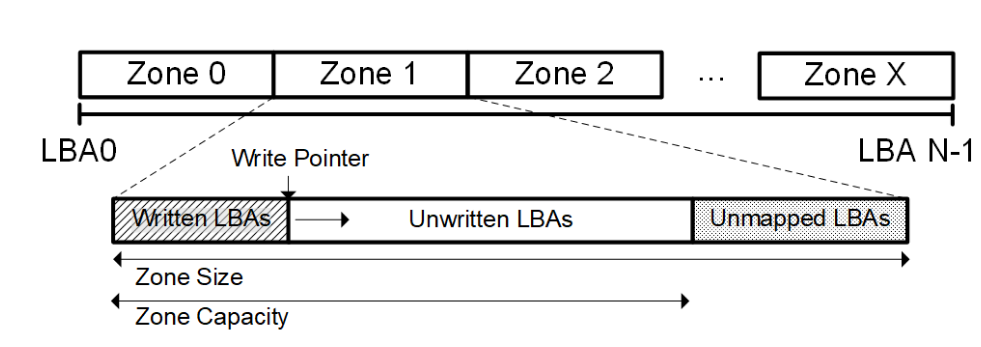
\includegraphics[width=0.8\textwidth]{fig/zns}
    \caption{单个 Zone 内的写逻辑}
    \label{zns}
\end{figure}

硬件方面的尝试其实不止 ZNS 一种。在利用硬件进行 SSD 存储优化的赛道上,有过许多新奇的软硬件技术。Intel 的傲腾就是其中之一,它利用全新的 3D XPoint 相变存储介质,将 SSD 的读写性能提升到了一个新的高度。但是傲腾的缺点也很明显,那就是成本高昂,而且只有 Intel 自家的 CPU 才能够完全发挥傲腾的性能。而 ZNS 和 Zoned Storage SSD 的优势在于,它们是 NVMe 的标准,任何厂商都可以按照标准来生产。而且 ZNS 和 Zoned Storage SSD 的实际生产成本并不高,硬件上主控的计算压力减少了,也释放了更多原来的预留空间,所以大量生产后成本会比现在的 SSD 还要低,因此在可以遇见的未来,ZNS SSD 还会更加普及。

除了傲腾,还有 Open-Channel SSD(OCSSD)。它的主要优化点在于,它将 SSD 的主控和垃圾回收的功能都放到了主机上,而 SSD 只负责读写数据。这样做的好处是,主机可以根据自己的应用场景来优化 SSD 的性能,而且 SSD 的成本也会降低。但是这样做的缺点也很明显,那就是主机的计算压力会变大,而且主机的应用场景也会受到限制。它与 Zoned Storage SSD 的区别主要在于,OCSSD 是将 FTL 放置在主机端,从而减小 SSD 上主控的 DRAM 成本等,而 Zoned Storage SSD 则干脆基本放弃了细粒度的 FTL,只在非常大的 Zone 粒度上做了大块逻辑映射和磨损均衡,从而进一步地让 SSD 服务于计算和存储本身。

\label{zone-type}

在硬件实现上,Zoned Storage SSD 可以设置 Zone 的类型。Zone 可以分为两类:Seq Zone 和 Conv Zone。Seq Zone 正如之前介绍的一样,可以随机读取,但是只能从指定的写指针位置写入数据。而 Conv Zone 则基本可以看作是普通的 SSD,主控仍然会维护这部分地址的 FTL ,所以这部分 Zones 可以像传统 SSD 一般随机读写。这样分类 Zones,更多地是为了兼容现有的应用场景,因为现有的应用场景中,随机读写的需求还是非常多的。而 Seq Zone 则是为了更好地适应新的应用场景,因为新的应用场景中,随机读写的需求并不多,而且 Seq Zone 的性能也更好。

软件方面,ZenFS 则是利用 RocksDB 的文件系统接口将文件放置到原始分区块设备上的区域中。

RocksDB 是 Facebook 开源的一个 KV 存储引擎,它是 LevelDB 的一个分支,主要用于存储 Facebook 的消息系统的元数据。RocksDB 的特点是,它是一个基于 LSM-Tree 的存储引擎,它的读写性能都非常高,而且它的写入放大也非常低。RocksDB 的写入放大主要是通过将写入的数据放到内存中的 MemTable 中,然后再将 MemTable 中的数据写入到磁盘中的 SSTable 中来实现的。RocksDB 的读写性能和写入放大都非常优秀,所以它在 Facebook 的消息系统中得到了广泛的应用。

RocksDB 的 LST-Tree 有多个层次,每个层次都有自己的 SSTable。在 RocksDB 中,每个 SSTable 都是一个文件,而每个 SSTable 中的数据都是有序的。在 RocksDB 中,每个 SSTable 都有一个大小的限制,当 SSTable 的大小达到限制时,就会将达到大小的 SSTable 进行 Compact 操作。LSM-Tree 的操作逻辑(图 \ref{lsm-tree} ),让这种数据结构在磁盘上的表现为一种类似于日志的结构,这样结构的数据库在磁盘上的随机写性能非常高,而且写入放大也非常低。

\begin{figure}[htbp]
    \centering
    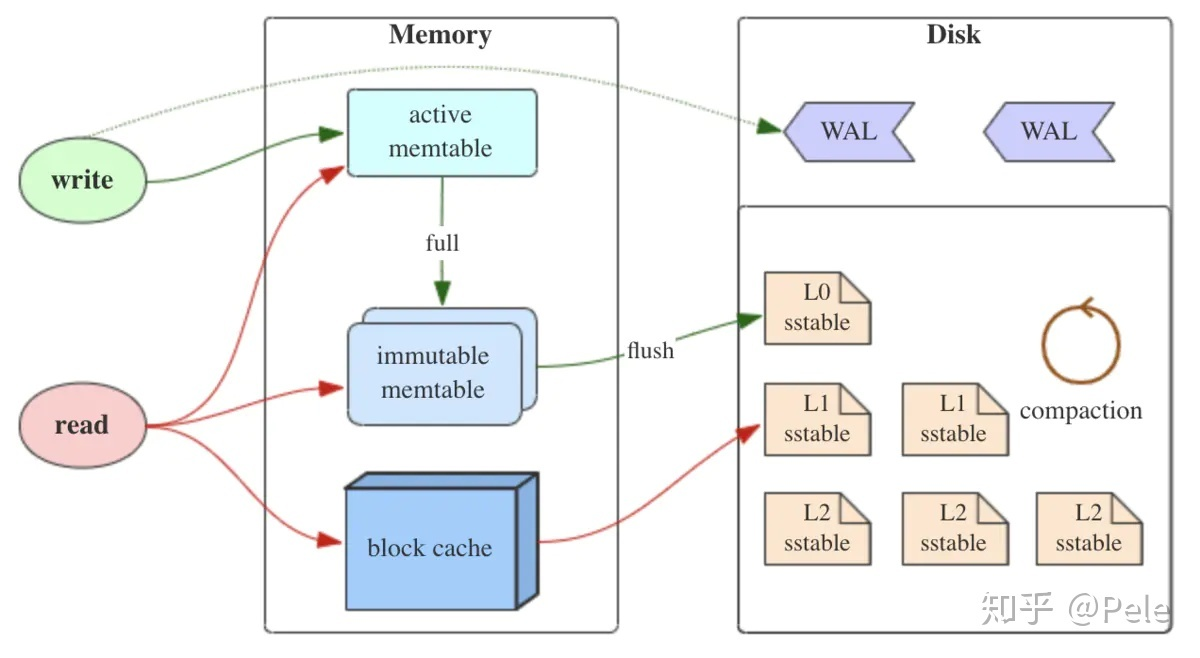
\includegraphics[width=0.8\textwidth]{fig/lsm-tree}
    \caption{LSM-Tree 的操作逻辑}
    \label{lsm-tree}
\end{figure}

在 ZenFS 中,每个上述提到的 SSTable 就是一个 \verb|.sst| 文件。ZenFS 对 SST 文件的管理,也如 SSTable 的完全追加写入如出一辙,即使用 WAL(Write Ahead Log)管理文件的 MetaData 和文件数据,甚至文件的重命名、修改、新增和删除,都是只追加写入的。

\subsubsection{ZenFS 源码分析}

在调研过程中,我们对 ZenFS 的源代码进行了一次完整的分析,总结出我们理解中的 ZenFS 的系统框图(图 \ref{zenfs} )。

\begin{figure}[htbp]
    \centering
    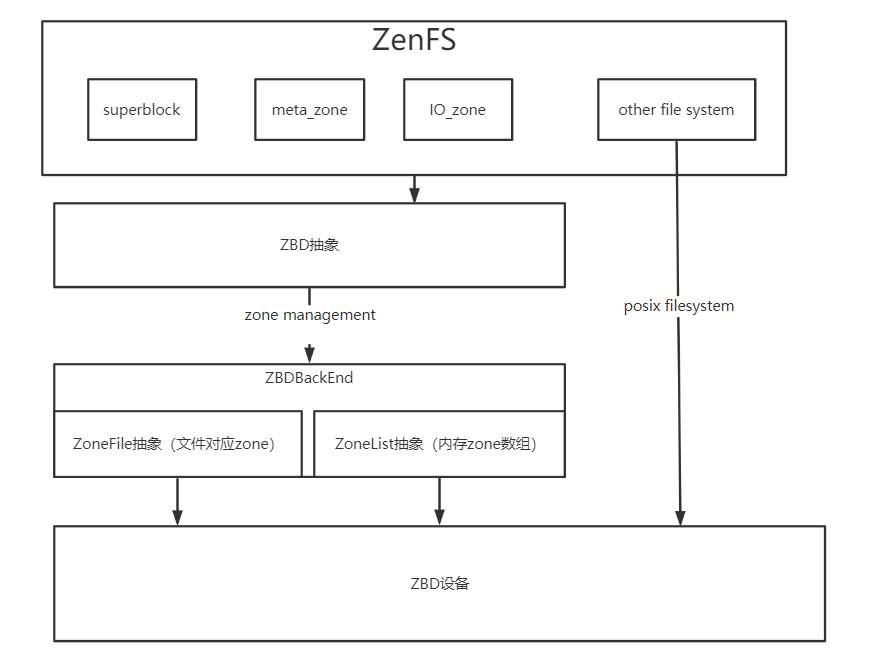
\includegraphics[width=0.8\textwidth]{fig/zenfs}
    \caption{ZenFS 系统框图}
    \label{zenfs}
\end{figure}

\subsubsubsection{Zone}

\begin{lstlisting}
  class Zone {
    ZonedBlockDevice *zbd_;
    ZonedBlockDeviceBackend *zbd_be_;
    std::atomic_bool busy_;
    
    uint64_t start_;//起始物理地址
    uint64_t capacity_; /* remaining capacity */
    uint64_t max_capacity_;
    uint64_t wp_;
    Env::WriteLifeTimeHint lifetime_;
    std::atomic<uint64_t> used_capacity_;
  }  
\end{lstlisting}

这里的 Zone 对应的就是设备上的 Zone,不过在 ZenFS 所管理的 Zones 中,只支持 Seq Zone,所以这里的 Zone 也只会是 Seq Zone。

一个Zone需要有所属块设备,起始地址和写指针,生命周期和空间相关的维护。
Zone中的方法有重置Zone,判断是否为空或者是否写满,往写指针后面添加数据等等。

\subsubsubsection{ZoneList}

\begin{lstlisting}
  class ZoneList {
    private:
     void *data_;
     unsigned int zone_count_;
   }   
\end{lstlisting}

由于一个 Zoned Storage SSD 上的 Zone 一般比较大,Zone 的数量并不多,所以 ZenFS 要求数据后端要能够快速地提供一个指向 Zones 信息列表的指针,然后通过这个指针就可以快速地求取 Zones 的信息,例如某个 Zone 的起始地址、容量、写指针、是否下线、是否显式打开等。

\subsubsubsection{ZonedBlockDeviceBackend}

ZonedBlockDeviceBackend是用来和底层设备交互需要经过的接口,这个接口将底层的ZoneList全部抽象成内存中连续的ZoneList并进行操作。

在 \verb|zbdlib_zenfs.h| 以及 \verb|zbdlib_zenfs.cc| 实现接口以方便上层对底层zbd的访问。

在\verb|zonefs_zenfs.h|以及\verb|zonefs_zenfs.cc|的实现是将上层对zbd的访问通过posix的读写文件方式给包装起来,从而能够访问到被 ZoneFS 包装过后的实际的 Zone。

\begin{lstlisting}
  class ZonedBlockDeviceBackend {
    public:
     uint32_t block_sz_ = 0;
     uint64_t zone_sz_ = 0;
     uint32_t nr_zones_ = 0;
   }   
\end{lstlisting}

backend有两种类型分别是:

\begin{lstlisting}
  enum class BackendType {
    kBlockDev,
    kZoneFS,
  };
\end{lstlisting}

当然,在我们实现了 RAID 之后,这里添加了 backend 类型 kRAID,用来表示这个 backend 是一个 被 RAID 后的数据后端。

\subsubsubsection{ZonedBlockDevice}

\begin{lstlisting}
  class ZonedBlockDevice {
    private:
     std::unique_ptr<ZonedBlockDeviceBackend> zbd_be_;
     std::vector<Zone *> io_zones;//用于io的zone
     std::vector<Zone *> meta_zones;//用于保存元信息的zone
     time_t start_time_;
     std::shared_ptr<Logger> logger_;
     uint32_t finish_threshold_ = 0;
     std::atomic<uint64_t> bytes_written_{0};
     std::atomic<uint64_t> gc_bytes_written_{0};// 垃圾回收转移的字节数目
   
     std::atomic<long> active_io_zones_;//分配io_zone时需要用锁
     std::atomic<long> open_io_zones_;
     /* Protects zone_resuorces_  condition variable, used
        for notifying changes in open_io_zones_ */
     std::mutex zone_resources_mtx_;
     std::condition_variable zone_resources_;
     std::mutex zone_deferred_status_mutex_;
     IOStatus zone_deferred_status_;
   
     std::condition_variable migrate_resource_;
     std::mutex migrate_zone_mtx_;
     std::atomic<bool> migrating_{false};
   
     unsigned int max_nr_active_io_zones_;
     unsigned int max_nr_open_io_zones_;
   
     std::shared_ptr<ZenFSMetrics> metrics_;//todo
   }   
\end{lstlisting}

\textbf {Open函数}

用来打开一个ZonedBlockDevice,流程如下:

\begin{itemize}
  \item 首先获取最大活跃io\_zones数目和最大可打开io\_zones,这里保留了几个zone用于metadata存储,一个额外的Zone用于extent migration,即Extent合并时使用的辅助空间。
  \item 从backend中获取已有zones分配3个meta\_zones。将剩余的非离线状态的可获得的zone放入io\_zones中。遍历的过程可统计当前活跃zone的数目。
\end{itemize}

处于离线状态的块,也就是offline,指的是这些块已经在硬件层面检测到错误,不可用了,需要被替换掉。

\textbf {Get*Space函数}:顾名思义,用来获取诸如已经使用空间,空闲空间以及可回收空间大小

\textbf {Log*函数}:用来输出日志,获取zone的整体使用情况,每个zone单个使用情况以及垃圾空间占比等。

\textbf {分配zone区域方法}

ZonedBlockDevice重要的功能应该是操作zone,其分配释放相关操作:

\begin{itemize}
\item ApplyFinishThreshold将剩余空间小于预设的块给finish掉,finish操作指的是把一个zone的写指针移动到zone末尾,剩余容量减为0。
\item FinishCheapestIOZone将一个最小剩余空间的zone给finish。
\item GetBestOpenZoneMatch将一个当前的文件生命周期和每一个io\_zone进行生命周期对比,分配一个生命周期大于当前文件的生命周期且最接近的zone。
\item AllocateEmptyZone,顾名思义是分配一块空的zone。
\item ReleaseMigrateZone,顾名思义是释放migrate\_zone (todo migrate zone是用来干嘛的)。
\item TakeMigrateZone,选择一块最优zone当作migrate\_zone。
\item AllocateIOZone,在保持max\_active\_io\_zones的数量的前提下分配一块zone。
\item Read,从偏移offset处读n个byte吧应该是,这里边用了ZonedDeviceBackend提供的Read接口。
\end{itemize}

而ZonedBlockDevice的读写数据,则基本直接调用ZonedBlockDeviceBackend的相关接口,即交给下一层处理。

\subsubsubsection{Snapshot}

ZenFS 的 Snapshot 功能,有多种存储结构的 Snapshot,其记录下某一个确定时间的各个结构的基本信息,从而实现 WAL 结构下的数据一致性保持和快照恢复功能。

几种 Snapshot 的存储结构如下:

\begin{lstlisting}
  // ZBD设备快照记录设备的空闲空间(free_space),已使用空间(used_space)和可回收空间(reclaimable_space)。
  class ZBDSnapshot {
    public:
     uint64_t free_space;//空闲空间
     uint64_t used_space;//已使用空间
     uint64_t reclaimable_space;//可回收空间
   }

   // Zone快照记录了Zone区域的开始地址(start),写指针(wp),以及容量相关信息。
   class ZoneSnapshot {
    public:
     uint64_t start;//Zone开始地址
     uint64_t wp;//写指针
   
     uint64_t capacity;//容量
     uint64_t used_capacity;//已用容量
     uint64_t max_capacity;//最大容量
   }
   class ZoneExtentSnapshot {
    public:
     uint64_t start;//todo
     uint64_t length;//Extent长度
     uint64_t zone_start;//todo
     std::string filename;//Extent所属文件名
   }
   // 论文中提到过一个文件拥有多个extent,extent不会跨Zone存储,在这些数据结构中可以看出。
   class ZoneFileSnapshot {
    public:
     uint64_t file_id;//顾名思义 file的id
     std::string filename;//文件名
     std::vector<ZoneExtentSnapshot> extents;//文件的extents快照集合
   }
   // 这里的快照便是之前所有快照的组合,记录了整个 ZenFS 设备的重要状态。
   class ZenFSSnapshot {
    public:
     ZBDSnapshot zbd_;
     std::vector<ZoneSnapshot> zones_;
     std::vector<ZoneFileSnapshot> zone_files_;
     std::vector<ZoneExtentSnapshot> extents_;
   };
   
\end{lstlisting}

\subsubsubsection{ZoneExtent}

ZoneFs的文件内容是由多个extent组成的,每个extent都放在一个zone里面,extent不能跨zone存储。

\begin{lstlisting}
  class ZoneExtent {
    public:
     uint64_t start_;// 物理起始地址
     uint64_t length_;// extent的长度
     Zone* zone_;// 所属zone指针
   
     explicit ZoneExtent(uint64_t start, uint64_t length, Zone* zone);
     Status DecodeFrom(Slice* input);
     void EncodeTo(std::string* output);
     void EncodeJson(std::ostream& json_stream);
   };   
\end{lstlisting}

\subsubsubsection{ZoneFile}

\begin{lstlisting}
  class ZoneFile {
    private:
     const uint64_t NO_EXTENT = 0xffffffffffffffff;
   
     ZonedBlockDevice* zbd_;
   
     std::vector<ZoneExtent*> extents_;
     std::vector<std::string> linkfiles_;
   
     Zone* active_zone_;
     uint64_t extent_start_ = NO_EXTENT;
     uint64_t extent_filepos_ = 0;
   
     Env::WriteLifeTimeHint lifetime_;
     IOType io_type_; /* Only used when writing */
     uint64_t file_size_;
     uint64_t file_id_;
   
     uint32_t nr_synced_extents_ = 0;
     bool open_for_wr_ = false;
     std::mutex open_for_wr_mtx_;
   
     time_t m_time_;
     bool is_sparse_ = false;
     bool is_deleted_ = false;
   
     MetadataWriter* metadata_writer_ = NULL;
   
     std::mutex writer_mtx_;// zonefs的读写锁
     std::atomic<int> readers_{0};
   
    public:
     static const int SPARSE_HEADER_SIZE = 8;
    }   
\end{lstlisting}

ZoneFile是ZenFS中的文件抽象,其记录了文件的元数据信息,包括文件名和路径、时间、文件id、文件大小、文件类型、文件的extents等。

zonefile在操作时只会操作一个active\_zone,同时文件记录了生命周期,读写锁等等。

其中实现的方法有稀疏文件append,所谓稀疏文件就是除了在zone中保存了有效数据信息之外还保存了有效数据的长度信息,如图 \ref{sparse-zone} 所示。

\begin{figure}[htbp]
  \centering
  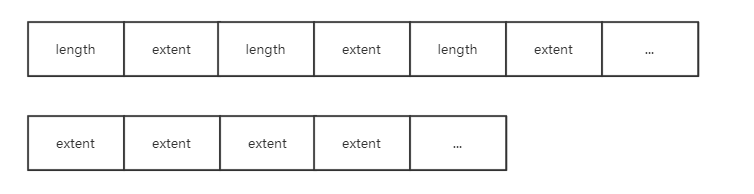
\includegraphics[width=0.8\textwidth]{fig/sparse_zone}
  \caption{ZoneFile 稀疏文件}
  \label{sparse-zone}
\end{figure}

sparse方式的zone中会将长度记录计入,而普通的zone只会一直append文件中的extent。sparse文件能够更加灵活地管理文件的空间,但是会比非sparse文件多一个长度字段信息。

除此之外,zonefs还有实现了RocksDB的FSWritableFile接口以支持顺序写的方法,实现了FSSequentialFile接口以实现顺序读,FSRandomAccessFile接口以实现随机读。

\subsubsubsection{SuperBlock}

\begin{lstlisting}
  class Superblock {
    uint32_t magic_ = 0;
    char uuid_[37] = {0};
    uint32_t sequence_ = 0;
    uint32_t superblock_version_ = 0;
    uint32_t flags_ = 0;
    uint32_t block_size_ = 0; /* in bytes */
    uint32_t zone_size_ = 0;  /* in blocks */
    uint32_t nr_zones_ = 0;
    char aux_fs_path_[256] = {0};
    uint32_t finish_treshold_ = 0;
    char zenfs_version_[64]{0};
    char reserved_[123] = {0};
   }  
\end{lstlisting}

ZenFS 的 SuperBlock 超级块相比其他文件系统的超级块要简单很多,其主要记录了一些基本信息,包括魔数、文件系统的版本、block的大小、zone的大小、zone的数量、辅助文件系统路径,之后大部分的信息都是保留字段。

ZenFS 的靠近实际硬件的设计使得它更加简洁高效,但是它的预留修改空间也留足了,为我们今后的修改优化提供了便利。我们全盘 RAID 的实现就是利用了它的超级块的预留空间。

\subsubsubsection{ZenMetaLog}

\begin{lstlisting}
  class ZenMetaLog {
    uint64_t read_pos_;
    Zone* zone_;
    ZonedBlockDevice* zbd_;
    size_t bs_;
  }  
\end{lstlisting}

ZenMetaLog 是 ZenFS 的元数据日志格式,是 ZenFS 非常重要的数据存储结构。

zenmetalog加入的record是如图\ref{meta_form}形式,首先存储的是由长度和数据形成的冗余码,然后是数据长度,再是实际的数据。

\begin{figure}[htbp]
  \centering
  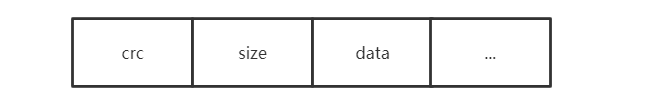
\includegraphics[width=0.8\textwidth]{fig/meta_form}
  \caption{ZenMetaLog Record}
  \label{meta_form}
\end{figure}

每一次roll的操作都会重新开一个zone来记录metadata信息,时机是当这个zone写满了todo,而一个新的metazone的内容首先会加入下面内容,此时记录的是文件系统的瞬时状态也即snapshot,当然这些snapshot是用record的形式加入的(图\ref{roll_metazone_init})。

\begin{figure}[htbp]
  \centering
  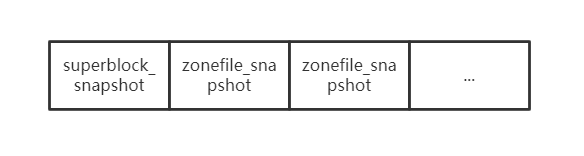
\includegraphics[width=0.8\textwidth]{fig/roll_metazone_init}
  \caption{ZenMetaLog Roll}
  \label{roll_metazone_init}
\end{figure}

在update,replace或是delete文件时,都会按照如图\ref{manipulate_form}格式包装成record加入metalog。

\begin{figure}[htbp]
  \centering
  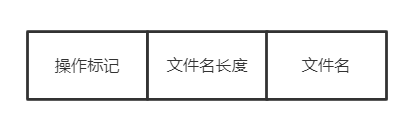
\includegraphics[width=0.8\textwidth]{fig/manipulate_form}
  \caption{ZenMetaLog 格式}
  \label{manipulate_form}
\end{figure}

\subsubsubsection{ZenFS}

\begin{lstlisting}
  class ZenFS : public FileSystemWrapper {
    ZonedBlockDevice* zbd_;
    std::map<std::string, std::shared_ptr<ZoneFile>> files_;// ZoneFile
    std::mutex files_mtx_;
    std::shared_ptr<Logger> logger_;
    std::atomic<uint64_t> next_file_id_;
  
    Zone* cur_meta_zone_ = nullptr;
    std::unique_ptr<ZenMetaLog> meta_log_;// 元信息
    std::mutex metadata_sync_mtx_;
    std::unique_ptr<Superblock> superblock_;// 超级块
  
    std::shared_ptr<Logger> GetLogger() { return logger_; }
  
    std::unique_ptr<std::thread> gc_worker_ = nullptr;// 垃圾回收
    bool run_gc_worker_ = false;
  }  
\end{lstlisting}

\textbf{GC\_WORKER垃圾回收}

当全局zone里边的free空间小于一定比例之后,gc\_worker便开始了垃圾回收工作,核心思想便是:

收集需要垃圾回收的zone,即zone的剩余空间满足一定的条件就进行回收,之后将zone中对应的extent移动到与当前zonefile生命周期相匹配的zone,这个zone是顺序写的,这个移动extent的操作叫做migrate操作。

ZenFS 内判断当前zone是否需要回收的条件还是比较简单的,是一个简单的容量判断。当文件系统 GC 时,找到超过容量的 Zone,再找到一个使用较少的 Zone,将超过容量的 Zone 中的数据迁移到使用较少的 Zone 中,就完成了一次 GC。这里ZenFS 简单的实现为我们之后的优化提供了便利。

\textbf{MOUNT逻辑}:

\begin{itemize}
  \item 读入所有metazone并且读出superblock,选择seq序号最大的superblock的meta作为恢复zone。
  \item 若是readonly的,则从磁盘同步一次数据。
  \item 若是可写的,并且用一个新的metazone记录当前文件系统的瞬时状态(superblock以及各个zonefile的编码)。同时要将系统的未用zone重置一下。最后开启垃圾回收线程。
\end{itemize}

\textbf{MKFS逻辑}:

\begin{itemize}
  \item 选择一个metazone作为log记录的zone。
  \item 写入superblock和各个zonfile编码到metazone中。
\end{itemize}

以上基本基于源码结构对 ZenFS 做了一个简单的分析。有了以上的理解分析,我们就可以开始对 ZenFS 进行修改优化了。